\documentclass[conference]{IEEEtran}
\IEEEoverridecommandlockouts
% The preceding line is only needed to identify funding in the first footnote. If that is unneeded, please comment it out.
\usepackage{cite}
\usepackage{amsmath,amssymb,amsfonts}
\usepackage{algorithmic}
\usepackage{graphicx}
\usepackage{textcomp}
\usepackage{xcolor}
\def\BibTeX{{\rm B\kern-.05em{\sc i\kern-.025em b}\kern-.08em
    T\kern-.1667em\lower.7ex\hbox{E}\kern-.125emX}}
\begin{document}

\title{Region-Aware ResNet-18 with Learnable Anatomical Embeddings for Facial Acne Severity Classification\\
%{\footnotesize \textsuperscript{*}Note: Sub-titles are not captured in Xplore and should not be used}
%\thanks{Identify applicable funding agency here. If none, delete this.}

}
\author{\IEEEauthorblockN{1\textsuperscript{st} Daniel C. Anselmo}
\IEEEauthorblockA{\textit{Dept. Pós-graduação (PPGCC-IFCE)} \\
\textit{Instituto Federal do Ceará (IFCE)}\\
Fortaleza, CE, Brazil \\
daniel.carvalho60@aluno.ifce.edu.br}
\and
\IEEEauthorblockN{2\textsuperscript{nd} Lucas G. Andrade}
\IEEEauthorblockA{\textit{Dept. de Telemática (DTEL)} \\
\textit{Instituto Federal do Ceará (IFCE)}\\
Fortaleza, CE, Brazil \\
gonluk0607@gmail.com}
\and
\IEEEauthorblockN{3\textsuperscript{nd} Enzo G. R. B. Moreira}
\IEEEauthorblockA{\textit{Dept. de Telemática (DTEL)} \\
\textit{Instituto Federal do Ceará (IFCE)}\\
Fortaleza, CE, Brazil \\
enzo.moreira62@aluno.ifce.edu.br}
\and
\IEEEauthorblockN{3\textsuperscript{rd} Dr. Pedro P. Rebouças Filho}
\IEEEauthorblockA{\textit{Dept. Pós-graduação (PPGCC-IFCE)} \\
\textit{Instituto Federal do Ceará (IFCE)}\\
Fortaleza, CE, Brazil \\
pedrosarf@ifce.edu.br}
\and
\IEEEauthorblockN{4\textsuperscript{th} Dr. Roger M. Sarmento}
\IEEEauthorblockA{\textit{Dept. Pós-graduação (PPGCC-IFCE)} \\
\textit{Instituto Federal do Ceará (IFCE)}\\
Fortaleza, CE, Brazil \\
rogerms@ifce.edu.br}

}


\maketitle

\begin{abstract}
Acne vulgaris is one of the most prevalent dermatological conditions worldwide, making the continuous assessment of its severity a significant challenge for teledermatology applications. Automated acne severity assessment represents a promising application of artificial intelligence to support teledermatology and remote patient monitoring. However, many existing approaches rely on computationally expensive architectures or multi-stage lesion detection, which often limits their implementation on mobile devices. This work proposes a region-aware framework in which five facial anatomical regions are automatically extracted using a landmark-based facial segmentation approach and classified by a lightweight, region-aware ResNet-18 network that incorporates learnable anatomical embeddings. The convolutional backbone is initialized in two stages, first on ImageNet and subsequently on a broader dermatological image collection, before fine-tuning on the acne severity task; the final model combines stochastic weight averaging, a multi-seed ensemble, and test-time augmentation. The proposed approach explicitly integrates anatomical context while maintaining a single, shared convolutional backbone, thereby reducing architectural complexity and computational cost. The model was evaluated on a combined image collection built from the public ACNE04 dataset and an independently sourced, author-annotated image set, for four-level acne severity classification. The evaluation includes a controlled ablation against a conventional ResNet-18 without anatomical embeddings, a cross-source generalization analysis, and an examination of regional performance. Under a fully leakage-controlled protocol, the proposed approach achieved 64.18\% accuracy and a weighted F1-score of 0.641; a controlled ablation shows comparable raw accuracy to a conventional ResNet-18 trained under an identical protocol, but a consistently higher Quadratic Weighted Kappa, indicating more ordinally consistent predictions in addition to the region-localized output that the conventional baseline cannot produce. A complementary whole-face baseline, trained under the same data and optimization protocol but without region segmentation, reached 76.26\% accuracy, indicating that the currently available data supports substantially higher accuracy when anatomical localization is not required and quantifying the accuracy currently traded for the region-level predictions that motivate the proposed design. An additional multi-region fusion variant, which combines all available region crops of the same image into a single prediction while still exploiting the learned anatomical embeddings, reached 69.06\% accuracy and a QWK of 0.770, recovering close to half of this gap without discarding anatomical structure, although at the cost of the per-region output that the region-crop model provides. Furthermore, a Flutter-based mobile prototype demonstrated the feasibility of integrating the proposed framework into teledermatology workflows. These results indicate that the proposed framework yields more ordinally consistent predictions than a region-agnostic baseline while additionally providing region-localized output, highlighting data diversity as the main direction for further gains in raw accuracy.
\end{abstract}
\begin{IEEEkeywords}
Acne vulgaris, acne severity classification, deep learning, ResNet-18, anatomical embeddings, teledermatology.
\end{IEEEkeywords}
\section{Introduction}
Acne vulgaris is one of the most prevalent inflammatory skin diseases worldwide, affecting approximately 85\% of adolescents and young adults. Beyond its dermatological manifestations, moderate to severe acne can lead to permanent scarring and significant psychosocial consequences that may impair quality of life, including anxiety, depression, and reduced self-esteem. Given that treatment efficacy depends on the continuous assessment of disease severity, frequent clinical monitoring is essential \cite{b1},\cite{b2}.

The growing advancements in teledermatology have expanded access to dermatological care by enabling the remote assessment of skin conditions via images captured with mobile devices \cite{b3},\cite{b4}. Concurrently, recent advances in Artificial Intelligence (AI) and Deep Learning (DL) have significantly enhanced the automated analysis of dermatological images, with convolutional neural networks (CNNs) achieving promising results in lesion detection, segmentation, and disease classification \cite{b5},\cite{b6}.

Despite advancements, the automated assessment of acne severity remains a challenge. Most existing approaches rely on multi-stage processing pipelines in which individual acne lesions are first detected and subsequently quantified to estimate disease severity \cite{b7} -\cite{b9}. Although effective, these strategies increase computational complexity, require lesion-level annotations, propagate errors across processing stages, and are less suitable for implementation on mobile devices. Furthermore, most previous studies evaluate model performance primarily based on global classification results under a single random split, with limited investigation into the isolated contribution of architectural design choices and generalization across independently collected data sources \cite{b10} -\cite{b12}.

To overcome these limitations, this work proposes a region-aware framework for classifying facial acne severity. The framework combines the automatic extraction of facial anatomical regions, using a landmark-based facial segmentation approach, with a lightweight, region-aware ResNet-18 network that incorporates learnable anatomical embeddings. This design explicitly integrates anatomical context while maintaining a single, shared convolutional backbone, thereby reducing computational complexity and facilitating implementation in teledermatology mobile applications.

The main contributions of this work are:
\begin{itemize}
\item The proposal of a Region-Aware framework that combines automatic anatomical facial region extraction with a lightweight Region-Aware ResNet-18 incorporating learnable anatomical embeddings for acne severity classification.
\item A controlled ablation study isolating the contribution of the anatomical embedding, comparing the proposed architecture against a conventional ResNet-18 trained under an identical data, backbone initialization, and optimization protocol, with results reported as mean $\pm$ standard deviation across multiple independent runs together with the corresponding ensemble performance.
\item A cross-source generalization analysis in which the model is trained on one image source and evaluated on the entirety of an independently collected, non-overlapping source, and vice versa, quantifying performance under real distribution shift rather than relying solely on a random split of a combined dataset.
\item The development of a Flutter-based mobile prototype demonstrating the feasibility of integrating the proposed framework into practical teledermatology workflows.
\end{itemize}

Thus, the proposed approach goes beyond the development of a classification model, integrating the automatic extraction of anatomical regions, AI-based inference, and implementation in a mobile application aimed at teledermatology applications.

The remainder of this paper is organized as follows. Section II reviews recent studies on AI-based acne severity assessment. Section III describes the proposed Region-Aware ResNet-18 architecture, datasets, and experimental protocol. Section IV presents the experimental results and discussion. Finally, Section V concludes the paper and outlines future research directions.

\section{Related Work}

\subsection{Automatic Acne Severity Assessment}
Recent advances in deep learning have significantly improved the automated assessment of acne severity from facial images. Existing approaches can be categorized into two groups: lesion-based multi-stage processing pipelines and direct severity classification models \cite{b13} -\cite{b16}.

Multi-stage approaches first detect individual acne lesions and then assess disease severity based on the number, type, or distribution of the detected lesions. Architectures based on Faster R-CNN, YOLO, and hybrid detection-and-classification frameworks have demonstrated competitive performance \cite{b13}–\cite{b17}. However, these approaches rely on detailed lesion-level annotations, entail higher computational costs, and make the classification process more sensitive to failures during the detection stage. These characteristics hinder their use in mobile applications, particularly in teledermatology scenarios requiring fast and efficient inference \cite{b11}, \cite{b12}.

Another approach involves direct classification models that estimate acne severity directly from facial images, without explicit lesion detection. CNN-based architectures, including ResNet, EfficientNet, and, more recently, CNN-Transformer and Vision Transformer models, have shown promising results while simplifying the inference process \cite{b15}–\cite{b18}, \cite{b21}. However, transformer-based models generally require greater computational resources, making their implementation on mobile devices more challenging. In contrast, lightweight CNNs, such as ResNet-18, offer a favorable balance between predictive performance, computational efficiency, and ease of implementation, characteristics that are desirable for teledermatology applications.



\subsection{Research Gap}
Despite the advances made in recent years, significant challenges remain regarding the widespread use of automated acne severity classification systems in teledermatology applications. Many proposed solutions achieve good experimental performance but rely on complex architectures, comprising multiple stages or various models, which increases computational cost and hinders their use on mobile devices. Furthermore, several approaches require detailed lesion annotations, making dataset creation more labor-intensive and limiting the scalability of these systems \cite{b14}, \cite{b19}–\cite{b21}.

Another aspect deserving attention is how these models are evaluated. Generally, studies focus their analysis on traditional performance metrics computed under a single random split, while aspects crucial for scientific rigor, such as the isolated contribution of a proposed architectural component and generalization across independently collected data sources, receive comparatively little attention \cite{b14}. In clinical applications, understanding whether a system generalizes beyond the population and acquisition conditions used for training is just as important as its average in-distribution performance.

Finally, few studies move beyond experimental evaluation to demonstrate the feasibility of deployment in real-world teledermatology scenarios. Model integration into mobile applications remains limited, despite the potential of these platforms to expand access to remote patient care and support the continuous monitoring of clinical progression \cite{b13}.

In contrast to these approaches, this paper presents a framework that utilizes a landmark-based facial segmentation approach exclusively during preprocessing to automatically locate anatomical facial regions, relying on a publicly available, pre-trained facial landmark estimator rather than a task-specific detector that would require its own annotated training set. Acne severity classification is subsequently performed by a lightweight, region-sensitive ResNet-18 network that incorporates learnable anatomical embeddings into a single shared convolutional backbone. This strategy preserves explicit anatomical context without relying on lesion-level annotations, multiple specialized models, or computationally expensive attention mechanisms. Furthermore, the proposed evaluation isolates the contribution of the anatomical embedding through a controlled ablation and quantifies generalization across independently collected image sources, alongside the implementation of a mobile prototype developed in Flutter \cite{b28} for teledermatology applications.




\section{Materials and Methods}
The proposed framework performs automatic classification of facial acne severity by combining anatomical information from the face. Instead of analyzing the face as a single image, the method first identifies key facial anatomical regions and then incorporates this information into the classification process using learnable anatomical embeddings. Figure~\ref{fig1} summarizes the complete processing pipeline adopted in this work.

\begin{figure}[htbp]
    \centering
    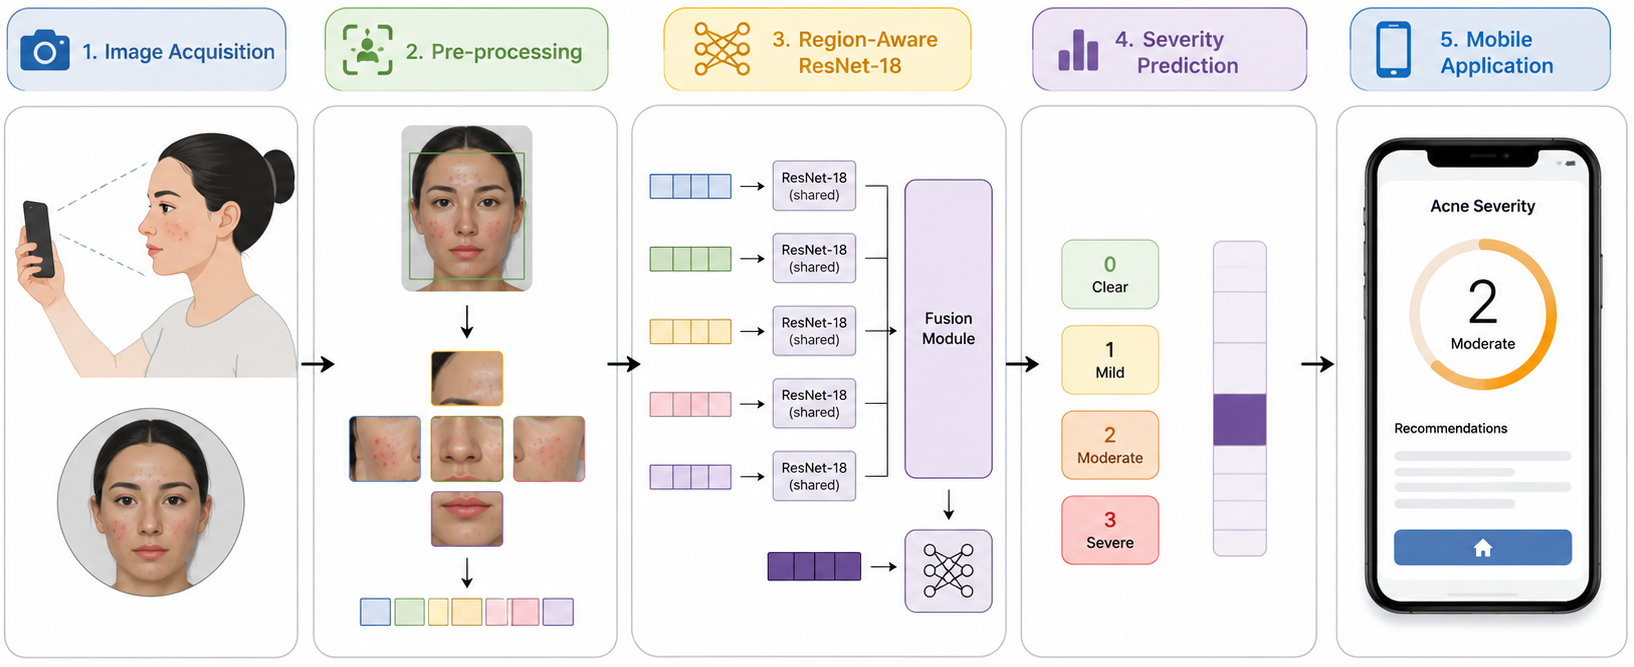
\includegraphics[width=\linewidth]{figures/fig1_.png}
    \caption{Overview of the proposed Region-Aware acne severity assessment pipeline.}
    \label{fig1}
\end{figure}

Initially, facial images are pre-processed and divided into their key anatomical regions. Next, each region is analyzed by the proposed Region-Aware ResNet-18 architecture, which combines visual features with learnable anatomical embeddings to estimate the acne severity level. Finally, the trained model is integrated into a mobile application developed in Flutter, enabling its use in teledermatology scenarios.

The remainder of this section is organized as follows. Section \ref{sub-III-a} describes the image sources and the processing pipeline, including the sampling unit adopted throughout the study. Section \ref{sub-III-b} presents the proposed Region-Aware ResNet-18 architecture. Section \ref{sub-III-c} details the training strategy, including backbone initialization, data augmentation, and optimization procedures, and finally, Section \ref{sub-III-d} describes the experimental protocol adopted to evaluate the proposed framework, including the ablation and cross-source generalization design.

\subsection{Image Sources, Sampling Unit, and Pre-processing}\label{sub-III-a}
The proposed framework was evaluated using a combined image collection built from two sources: the public ACNE04 dataset \cite{b27} and an independently collected image set annotated by one of the authors (referred to hereafter as the \textit{author-annotated} collection). The author-annotated collection aggregates facial images gathered from multiple public sources not previously labeled for severity; each image was graded and subsequently reviewed by the same annotator, following the same four-level Hayashi severity scale \cite{b12} used in ACNE04. Unlike ACNE04, this collection originates from a distinct population and image acquisition conditions (cameras, framing, and lighting), which allows it to be used both to enlarge the training collection and, separately, as an independent source for the cross-source generalization analysis described in Section \ref{sub-III-d}. Table~\ref{tab1} summarizes the two image sources.

\begin{table}[htbp]
\centering
\caption{Characteristics of the image sources used in this study}
\label{tab1}
\small
\begin{tabular}{|p{2.6cm}|p{2.6cm}|p{2.6cm}|}
\hline
\textbf{Characteristic} & \textbf{ACNE04} & \textbf{Author-annotated} \\
\hline
Images                  & 1,216           & 790              \\
\hline
Classes                 & 4               & 4                  \\
\hline
Severity Scale          & Hayashi (0–3)   & Hayashi (0–3)      \\
\hline
Annotators        & Original dataset labels & Single annotator (author), self-reviewed \\
\hline
\end{tabular}
\end{table}

It is important to clarify the sampling unit adopted throughout this work, since each source image yields multiple anatomical region crops and, consequently, may contribute more than one sample to training and evaluation. The combined image collection comprises 2,006 unique facial images. Each image is automatically segmented into up to five anatomical region crops (forehead, chin, nose, left cheek, and right cheek); crops that fail a minimum size or sharpness criterion are discarded, so a given image may contribute between one and five valid crops. This process yields 7,653 region crops in total, which constitute the actual samples used to train and evaluate the classification model, since the proposed architecture classifies one anatomical region crop at a time. All training, validation, and test set sizes reported in this paper refer to this region-crop sampling unit unless explicitly stated as unique images. The split into training (70\%), validation (15\%), and test (15\%) subsets was performed at the image level, prior to region segmentation, so that every crop originating from the same source image is assigned to the same subset, preventing any individual from appearing in more than one subset. This split is additionally verified after every dataset update to guarantee the absence of cross-subset duplicates.

The preprocessing pipeline is illustrated in Fig.~\ref{fig2}. First, a landmark-based facial segmentation approach, built on a 478-point facial mesh estimator, was used to automatically locate five facial anatomical regions (forehead, chin, nose, left cheek, and right cheek) instead of relying on a single global facial bounding box. A fixed subset of anatomical landmarks is used to derive each region's bounding box, based on well-established, publicly available facial landmark detection, requiring no additional detector training. This approach allows the model to explore visual features specific to each region.
\begin{figure}[htbp]
    \centering
    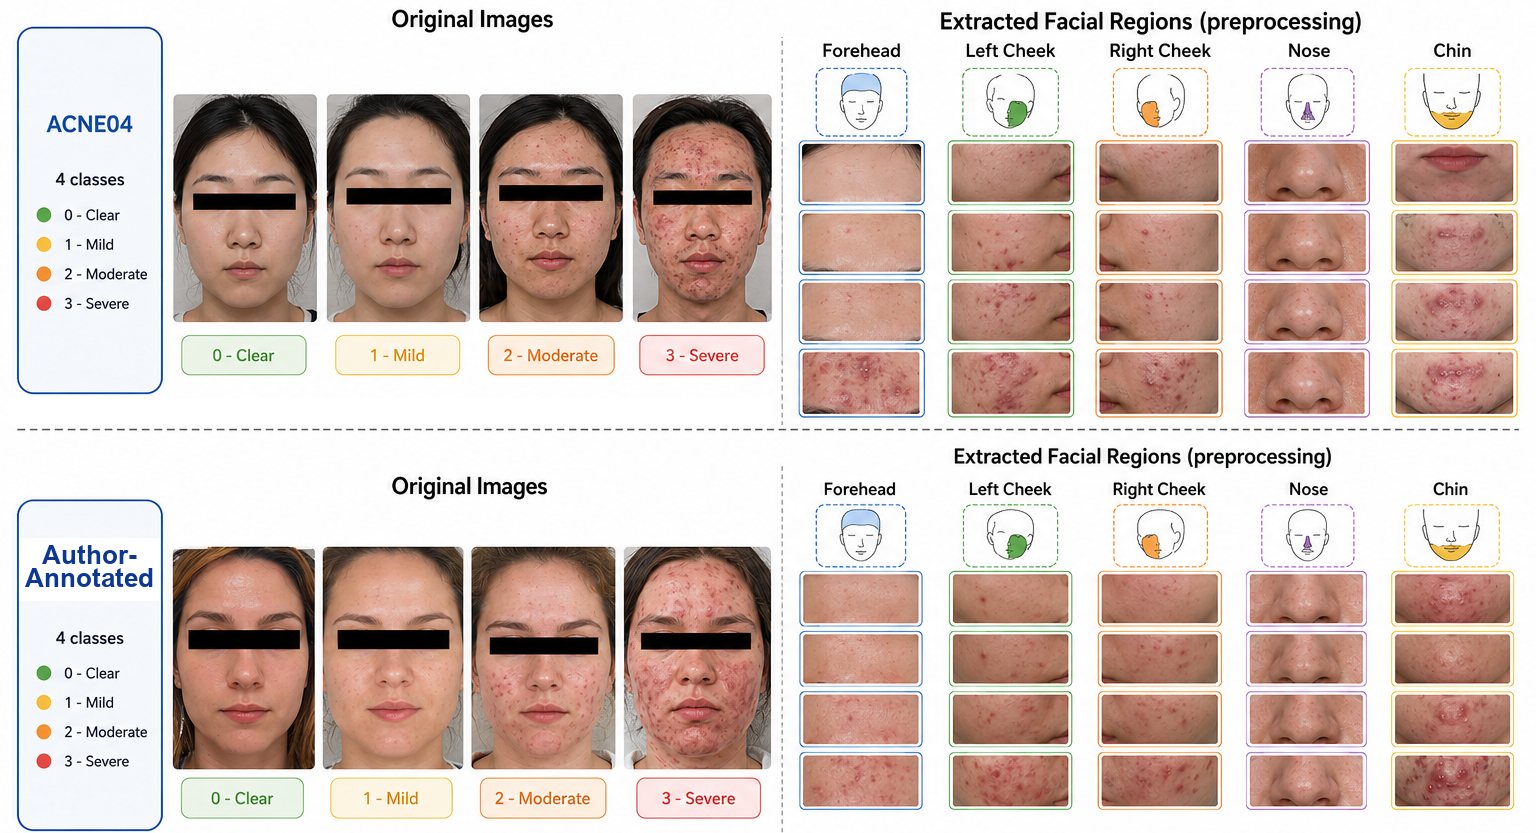
\includegraphics[width=\linewidth]{figures/fig2_.png}
    \caption{Samples of the datasets and the five automatically extracted facial anatomical regions.}
    \label{fig2}
\end{figure}

Each extracted region was resized to 224 × 224 pixels and normalized to ensure a standardized input for the classification model. Figure~\ref{fig2} illustrates representative facial images together with the corresponding anatomical regions obtained after the preprocessing stage.


\subsection{Proposed Region-Aware ResNet-18}\label{sub-III-b}
The proposed Region-Aware ResNet-18 is the core classification module of the proposed framework. After the preprocessing stage, each anatomical facial region is processed independently by the network. As illustrated in Fig.~\ref{fig3}, the model receives two inputs: a cropped facial region image and its corresponding anatomical region index, which is used to retrieve the learnable embedding associated with that anatomical location.

\begin{figure}[htbp]
    \centering
    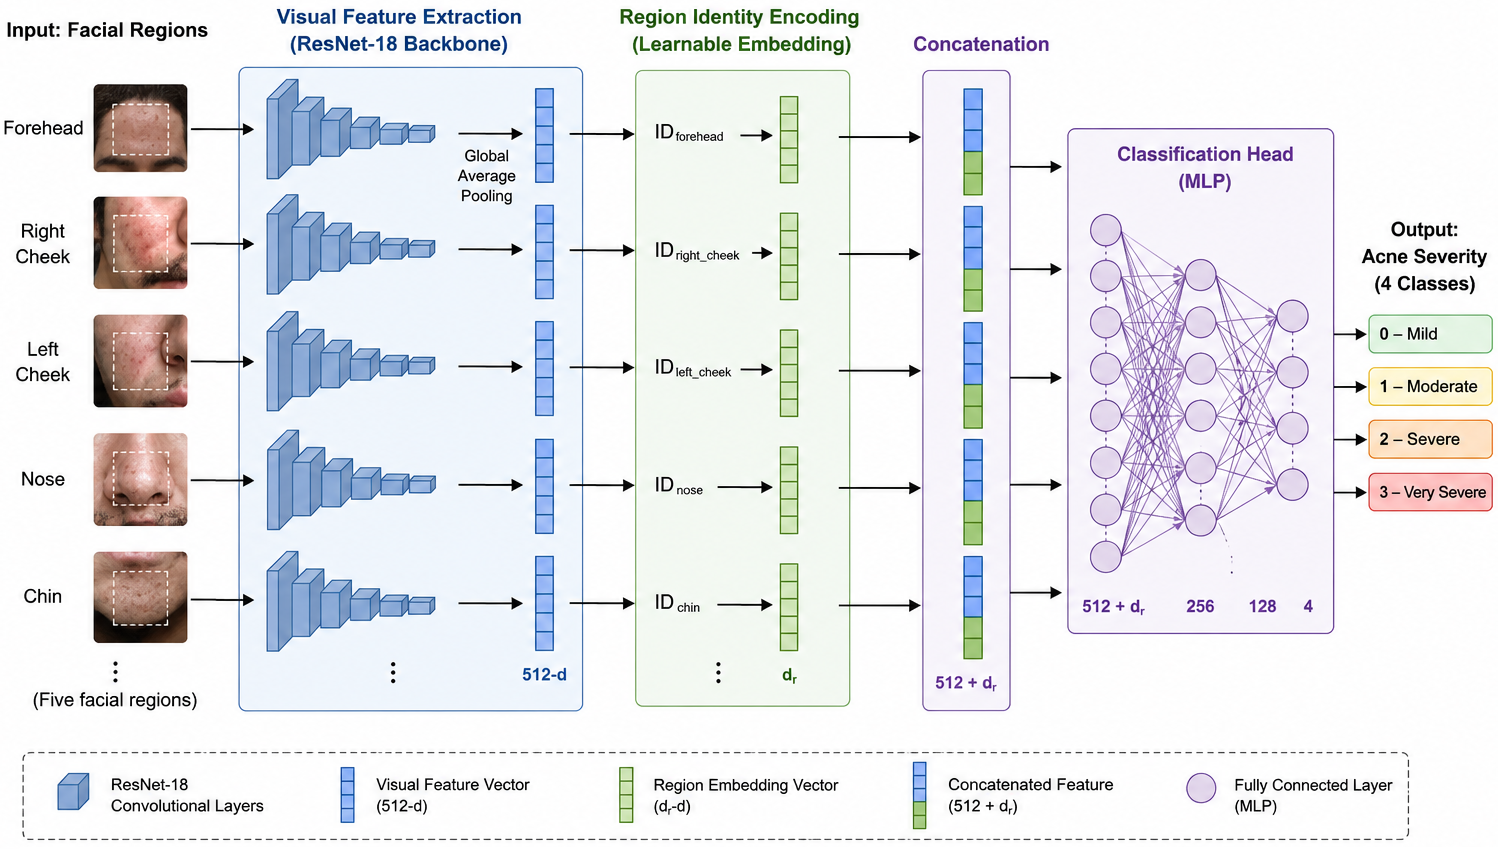
\includegraphics[width=\linewidth]{figures/fig3_.png}
    \caption{Proposed Region-Aware ResNet-18 architecture.}
    \label{fig3}
\end{figure}

Let $\mathbf{x}_r$ denote the cropped image corresponding to anatomical region $r$, where $r\in\{1,\ldots,R\}$ and $R=5$ represents the five facial regions considered in this study.

Visual features are extracted by a ResNet-18 backbone, represented by $\phi(\cdot)$. After the convolutional layers and the Global Average Pooling (GAP) operation, the network produces a visual feature vector given by

\begin{equation}
\mathbf{f}_r=\phi(\mathbf{x}_r),
\label{eq:visual_features}
\end{equation}

where $\mathbf{f}_r\in\mathbb{R}^{512}$ denotes the visual feature vector extracted from facial region $r$.

To explicitly incorporate anatomical information, each facial region is associated with a learnable embedding. The embedding matrix is defined as

\begin{equation}
\mathbf{E}\in\mathbb{R}^{R\times d},
\label{eq:embedding_matrix}
\end{equation}

where $R=5$ denotes the number of anatomical regions and $d=64$ is the embedding dimension. The embedding corresponding to region $r$ is obtained as

\begin{equation}
\mathbf{e}_r=\mathbf{E}[r],
\label{eq:region_embedding}
\end{equation}

where $\mathbf{e}_r\in\mathbb{R}^{64}$ encodes the anatomical identity of the input region.

The visual feature vector and the corresponding anatomical embedding are then concatenated to produce the final feature representation,

\begin{equation}
\mathbf{z}_r=
\mathbf{f}_r
\oplus
\mathbf{e}_r,
\label{eq:fusion}
\end{equation}

where $\oplus$ denotes vector concatenation. Since $\mathbf{f}_r\in\mathbb{R}^{512}$ and $\mathbf{e}_r\in\mathbb{R}^{64}$, the resulting representation belongs to $\mathbb{R}^{576}$.

The fused representation is processed by a classification head composed of fully connected layers, Batch Normalization, ReLU activation, and Dropout regularization,

\begin{equation}
\mathbf{o}_r=g(\mathbf{z}_r),
\label{eq:classifier}
\end{equation}

where $g(\cdot)$ denotes the classification head and $\mathbf{o}_r\in\mathbb{R}^{C}$ contains the logits associated with the $C=4$ acne severity classes.

Class probabilities are computed using the Softmax function,

\begin{equation}
p_{r,c}=
\frac{\exp(o_{r,c})}
{\sum_{k=1}^{C}\exp(o_{r,k})},
\label{eq:softmax}
\end{equation}

and the predicted severity level is obtained by

\begin{equation}
\hat{y}_r=
\arg\max_c p_{r,c}.
\label{eq:prediction}
\end{equation}

Unlike a conventional ResNet-18, the proposed architecture incorporates the anatomical identity of each facial region into the classification process through learnable embeddings. This allows the network to adapt its feature representation based on the anatomical context while maintaining a single, shared backbone structure for all facial regions. Consequently, the proposed approach learns region-specific visual patterns with only a slight increase in the number of trainable parameters (approximately 0.1\% of the backbone's total parameter count), preserving the simplicity and computational efficiency of the original architecture. These characteristics make the proposed model suitable for integration into mobile teledermatology applications. Section \ref{sub-IV-b} reports a controlled ablation in which this same architecture is trained with the embedding branch removed, isolating its measured contribution.

\subsection{Training Strategy}\label{sub-III-c}

The proposed framework was trained in a supervised multi-class classification scenario, employing a Weighted Cross-Entropy loss function to mitigate the impact of class imbalance during optimization. Model parameters were updated using the Adam optimizer, which ensured stable convergence throughout the training process.

The convolutional backbone was initialized in two stages prior to fine-tuning on the acne severity task. It was first initialized with ImageNet-pretrained weights and subsequently fine-tuned on the Skin Condition Image Network (SCIN) dataset, a broader collection covering general dermatological conditions, allowing the network to learn generic skin-texture representations before specializing in acne severity grading.

To enhance the model's generalization capability, several data augmentation techniques were applied during training, including random horizontal flipping, rotations, color jittering, Gaussian blurring, Random Erasing, and mixup interpolation between training samples. Furthermore, the learning rate was dynamically adjusted using the ReduceLROnPlateau scheduler, while early stopping was adopted to prevent overfitting and preserve the best-performing model.

After convergence under early stopping, the model was further refined using Stochastic Weight Averaging (SWA) \cite{b29}: training continued for a fixed number of additional epochs at a reduced, constant learning rate, and the final weights were obtained by averaging the model parameters across these epochs, followed by a recalibration of the Batch Normalization statistics. The final reported model combines an ensemble of independently trained instances, each initialized with a different random seed, together with test-time augmentation (TTA): at inference time, each test crop is evaluated under a small set of augmented views, and the predicted class probabilities are averaged across both the ensemble members and the augmented views before the final decision is taken.

The framework was implemented using PyTorch \cite{b24}. The key hyperparameters adopted during training are summarized in Table~\ref{tab2}. \begin{table}[htbp]
\caption{Main hyperparameters used during the training of the proposed architecture.}
\begin{center}
\small
\begin{tabular}{|l|p{4.8cm}|}
\hline
\textbf{Parameter} & \textbf{Value} \\
\hline
Framework & PyTorch \\
\hline
Backbone & ResNet-18 \\
\hline
Backbone initialization & ImageNet $\rightarrow$ SCIN \\
\hline
Optimizer & Adam \\
\hline
Loss function & Weighted Cross-Entropy \\
\hline
Learning rate & 0.0001 \\
\hline
Scheduler & ReduceLROnPlateau \\
\hline
Batch size & 16 \\
\hline
Maximum epochs & 40 (+10 SWA epochs) \\
\hline
Data augmentation & Horizontal flip ($p=0.5$), Rotation ($\pm25^\circ$), Color Jitter, Gaussian Blur, Random Erasing, Mixup ($\alpha=0.2$) \\
\hline
Regularization & Batch Normalization and Dropout \\
\hline
Model refinement & Stochastic Weight Averaging \\
\hline
Ensemble & 5 independent seeds \\
\hline
Test-time augmentation & 7 views per sample \\
\hline
Hardware & Apple M-series (MPS backend) \\
\hline
\end{tabular}
\label{tab2}
\end{center}
\end{table}

These training strategies were selected to improve model robustness while maintaining a lightweight architecture suitable for practical implementation. Combined with the proposed anatomical embeddings, they contributed to stable convergence across the different facial regions evaluated in this study.

\subsection{Experimental Protocol}\label{sub-III-d}

The proposed framework was evaluated using standard multiclass classification metrics: Accuracy, Precision, Recall, and F1-score, together with the Quadratic Weighted Kappa (QWK), which accounts for the ordinal nature of the severity scale by penalizing errors between distant classes more heavily than errors between adjacent ones. These metrics are defined as follows:

\begin{align}
\mathrm{Accuracy} &= \frac{TP+TN}{TP+TN+FP+FN},\\
\mathrm{Precision} &= \frac{TP}{TP+FP},\\
\mathrm{Recall} &= \frac{TP}{TP+FN},\\
F_1 &= 2\cdot
\frac{\mathrm{Precision}\cdot\mathrm{Recall}}
{\mathrm{Precision}+\mathrm{Recall}}.
\end{align}

where $TP$, $TN$, $FP$, and $FN$ denote true positives, true negatives, false positives, and false negatives, respectively. Since acne severity classification involves four classes, Precision, Recall, and F1-score were computed for each class and reported using a weighted average.

Three complementary experiments were considered. \textit{(i) Overall and regional performance:} the proposed Region-Aware ResNet-18 is evaluated on the combined test set described in Section \ref{sub-III-a}, both overall and broken down by anatomical region. \textit{(ii) Ablation study:} to isolate the contribution of the proposed embedding, a conventional ResNet-18 (\textit{NoEmbed}), identical to the proposed architecture except for the removal of the embedding branch described in Section \ref{sub-III-b}, was trained under the exact same data, backbone initialization, augmentation, and optimization protocol as the proposed model (\textit{WithEmbed}). Both configurations were trained across 5 independent random seeds, and results are reported as mean $\pm$ standard deviation, together with the ensemble performance of each configuration. \textit{(iii) Cross-source generalization:} rather than relying solely on a random split of the combined image collection, generalization was additionally assessed across the two independently collected image sources described in Section \ref{sub-III-a}. In the first direction, the model is trained exclusively on ACNE04 and evaluated on the entire author-annotated collection; in the second direction, training and evaluation sources are reversed.

Together, these analyses provide a broader characterization of the proposed framework, evaluating not only its predictive performance but also the isolated contribution of its central architectural component and its ability to generalize across independently collected data.


\section{Experimental Results}
The experimental evaluation aims to investigate the proposed framework from different perspectives: overall and regional classification performance, the isolated contribution of the anatomical embedding, and generalization across independently collected image sources.

\subsection{Overall Classification Performance}
The overall classification performance of the proposed framework on the test set is summarized in Table~\ref{tab:metrics}. The proposed framework achieved an overall accuracy of 64.18\% and a weighted F1-score of 0.641, with a Quadratic Weighted Kappa of 0.718, under a fully controlled protocol in which the training, validation, and test subsets were verified to contain no duplicate or overlapping source images. Test-set support totals 1,061 region crops sampled from 278 unique test images, consistent with the sampling unit defined in Section \ref{sub-III-a}.
\begin{table}[htbp]
\caption{Overall classification performance of the proposed architecture.}
\begin{center}
\small
\begin{tabular}{|l|c|c|c|c|}
\hline
\textbf{Class} & \textbf{Precision} & \textbf{Recall} & \textbf{F1-score} & \textbf{Support} \\
\hline
Mild (0) & 0.64 & 0.69 & 0.66 & 356 \\
\hline
Moderate (1) & 0.65 & 0.60 & 0.62 & 441 \\
\hline
Severe (2) & 0.63 & 0.64 & 0.63 & 195 \\
\hline
Very Severe (3) & 0.63 & 0.70 & 0.66 & 69 \\
\hline
Weighted Average & 0.64 & 0.64 & 0.64 & 1061 \\
\hline
\textbf{Overall Accuracy} & \multicolumn{4}{l|}{64.18\% (QWK = 0.718)} \\
\hline
\end{tabular}
\label{tab:metrics}
\end{center}
\end{table}

The results show that the model maintained balanced performance across the four severity levels, with no class collapsing toward zero recall despite the natural class imbalance of the underlying data. Fig.~\ref{fig4} presents the row-normalized confusion matrix.

\begin{figure}[htbp]
    \centering
    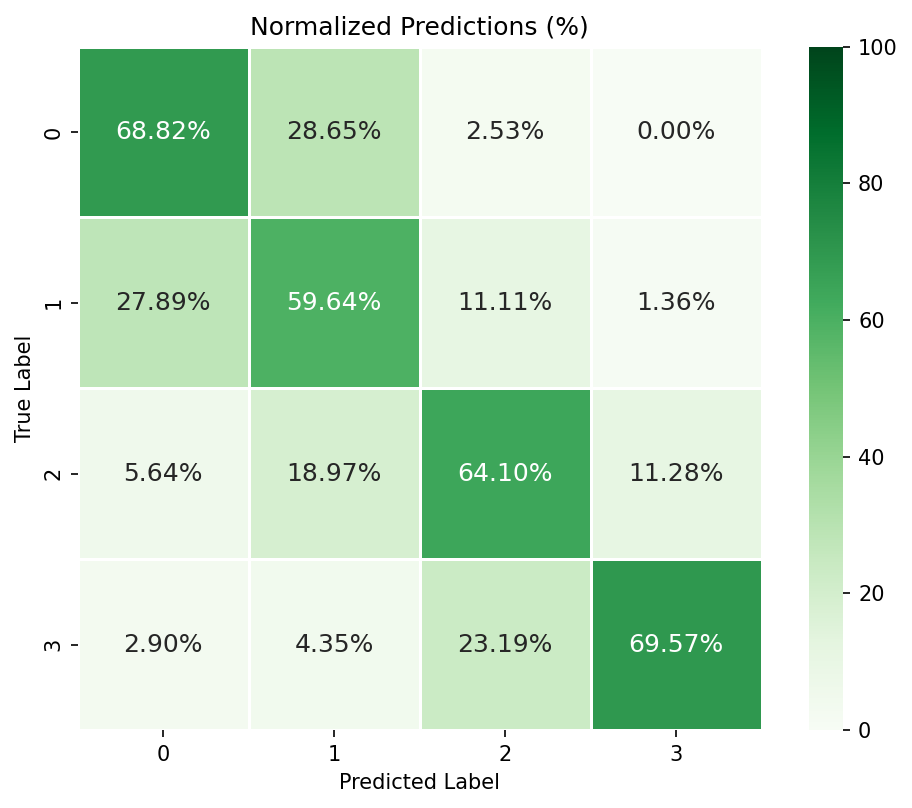
\includegraphics[width=\linewidth]{figures/fig4_.png}
    \caption{Row-normalized confusion matrix (\%) obtained on the test set for the proposed Region-Aware ResNet-18 (ensemble + TTA).}
    \label{fig4}
\end{figure}

Most classification errors occur between adjacent acne severity levels; confusion between the extreme classes (Mild and Very Severe) remains comparatively limited, indicating that prediction errors are primarily concentrated in clinically adjacent categories rather than distributed uniformly across the severity scale.

\subsection{Ablation Study: With vs. Without Anatomical Embeddings}\label{sub-IV-b}

To directly address whether the anatomical embedding contributes to classification performance, the proposed Region-Aware ResNet-18 (\textit{WithEmbed}) was compared against a conventional ResNet-18 (\textit{NoEmbed}) trained under an identical protocol, as described in Section \ref{sub-III-d}. Table~\ref{tab:ablation} reports the mean $\pm$ standard deviation across 5 independent seeds, together with the ensemble performance of each configuration.

\begin{table}[htbp]
\caption{Ablation study: Region-Aware ResNet-18 (WithEmbed) vs. conventional ResNet-18 (NoEmbed).}
\begin{center}
\small
\begin{tabular}{|l|c|c|c|}
\hline
\textbf{Configuration} & \textbf{Accuracy} & \textbf{F1} & \textbf{QWK} \\
\hline
NoEmbed (mean $\pm$ std) & 60.64\% $\pm$ 1.02 & 0.605 & 0.665 \\
\hline
WithEmbed (mean $\pm$ std) & 60.64\% $\pm$ 1.27 & 0.606 & 0.668 \\
\hline
NoEmbed (ensemble+TTA) & 64.18\% & 0.641 & 0.698 \\
\hline
\textbf{WithEmbed (ensemble+TTA)} & \textbf{64.18\%} & \textbf{0.641} & \textbf{0.718} \\
\hline
\end{tabular}
\label{tab:ablation}
\end{center}
\end{table}

Under an identical data, backbone initialization, and optimization protocol, the Region-Aware and conventional configurations achieved comparable raw accuracy and F1-score, both at the individual-seed level (60.64\% $\pm$ 1.27 vs. 60.64\% $\pm$ 1.02) and after ensembling (64.18\% vs. 64.18\%). The anatomical embedding did, however, yield a consistently higher Quadratic Weighted Kappa in both settings (0.668 vs. 0.665 per seed; 0.718 vs. 0.698 for the ensemble), indicating that its errors are more concentrated on ordinally adjacent severity levels rather than distributed further from the true class. Under the current data budget, the measured benefit of the proposed embedding is therefore not an increase in raw classification accuracy, but a more ordinally consistent error structure, together with the region-localized predictions that a conventional, region-agnostic classifier cannot produce by design.

\subsection{Cross-Source Generalization}

Table~\ref{tab:cross} reports the cross-source generalization results described in Section \ref{sub-III-d}. In each direction, the model is trained exclusively on one image source and evaluated on the entirety of the other, independently collected source.

\begin{table}[htbp]
\caption{Cross-source generalization performance.}
\begin{center}
\small
\begin{tabular}{|l|c|c|c|}
\hline
\textbf{Train} $\rightarrow$ \textbf{Test} & \textbf{Accuracy} & \textbf{F1} & \textbf{QWK} \\
\hline
ACNE04 $\rightarrow$ Author-annotated & 30.23\% & 0.287 & 0.199 \\
\hline
Author-annotated $\rightarrow$ ACNE04 & 25.55\% & 0.268 & 0.147 \\
\hline
\end{tabular}
\label{tab:cross}
\end{center}
\end{table}

Both directions show a substantial drop relative to the in-distribution result reported in Table~\ref{tab:metrics}, quantifying a real generalization cost that a single random split over the combined collection would otherwise obscure. Inspection of the per-class confusion pattern for the Author-annotated $\rightarrow$ ACNE04 direction reveals that the model does not fail uniformly at random: predictions are systematically biased toward the severity classes that dominate the training source, rather than the class distribution of the test source, an effect consistent with the substantially different photographic conditions (camera type, framing distance, and lighting) of the two collections. Rather than indicating a defect in the model, this pattern illustrates a well-documented failure mode of classifiers under covariate shift, in which the learned class prior does not transfer across sufficiently different acquisition domains. This result reinforces that continued diversification of the training collection across acquisition conditions, rather than architectural changes alone, is the most direct path toward narrowing this gap, and is discussed further in Section VI.

\subsection{Regional Performance Analysis}
One of the main contributions of the proposed architecture is the explicit incorporation of anatomical information through learnable facial region embeddings. To evaluate the effectiveness of this strategy, classification performance was analyzed independently for each facial region. Table \ref{tab4} presents the performance achieved for each facial region, considering the weighted metrics of Precision, Recall, and F1-score.
\begin{table}[htbp]
\caption{Weighted classification performance according to facial region.}
\begin{center}
\small
\begin{tabular}{|l|c|c|c|c|}
\hline
\textbf{Facial Region} & \textbf{Precision} & \textbf{Recall} & \textbf{F1-score} & \textbf{Support} \\
\hline
Forehead & 0.62 & 0.62 & 0.62 & 253 \\
\hline
Chin & 0.61 & 0.61 & 0.61 & 234 \\
\hline
Nose & 0.60 & 0.60 & 0.59 & 267 \\
\hline
Left Cheek & 0.74 & 0.73 & 0.73 & 166 \\
\hline
Right Cheek & 0.71 & 0.70 & 0.70 & 141 \\
\hline
\end{tabular}
\label{tab4}
\end{center}
\end{table}

Performance varies noticeably across facial regions, with weighted F1 scores ranging from 0.59 (nose) to 0.73 (left cheek). The left cheek yielded the strongest performance, while the nose was the most challenging region. This variability is consistent with differences in the amount and diversity of training samples available per region after the crop-quality filtering step described in Section \ref{sub-III-a}, and suggests that region-specific data availability, rather than the architecture itself, is the main driver of the residual regional gap. These results indicate that the proposed anatomical embeddings allow all facial regions to be processed by a single shared network without increasing architectural complexity, which is particularly advantageous for mobile teledermatology applications, while pointing to region-balanced data collection as a concrete direction for future improvement.

\subsection{Training Stability Across Independent Seeds}

Beyond point-estimate accuracy, it is important to verify that the proposed framework converges consistently across independent training runs rather than depending on a fortunate initialization. Figure~\ref{fig5} shows the test accuracy obtained by the WithEmbed configuration across the 5 independent seeds used for the ensemble reported in Table~\ref{tab:ablation}.

\begin{figure}[htbp]
    \centering
    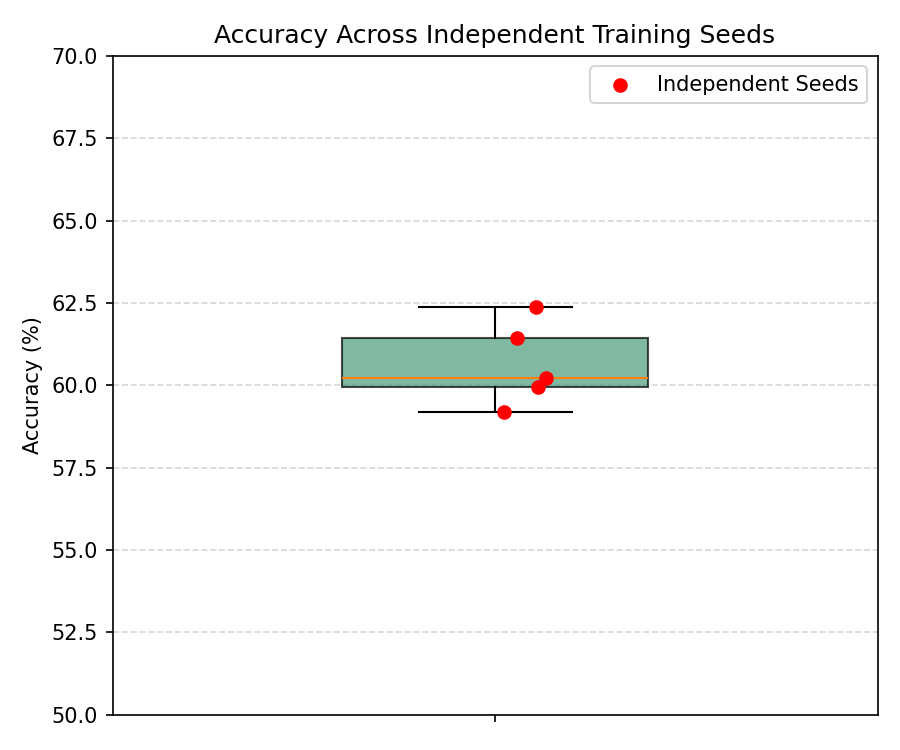
\includegraphics[width=\linewidth]{figures/fig5_.png}
    \caption{Test accuracy of the proposed architecture across independent training seeds (mean 60.64\%, standard deviation 1.27 percentage points).}
    \label{fig5}
\end{figure}

The observed standard deviation of 1.27 percentage points across seeds indicates that the model converges to a comparable solution regardless of random initialization, supporting the reliability of the reported ensemble result. A broader robustness analysis under varied acquisition conditions is discussed as future work in Section VI, given that the two image sources currently available do not yet span the full range of smartphone cameras and capture conditions expected in real-world teledermatology use.

\subsection{Whole-Face Baseline: Contextualizing the Region-Crop Ceiling}\label{sub-IV-f}

To contextualize the accuracy level reported in Table~\ref{tab:metrics}, a complementary baseline was trained on the same, leakage-verified image collection, but classifying each whole facial image directly (without region segmentation or anatomical embeddings), following the same backbone initialization, SWA, ensemble, and TTA protocol described in Section \ref{sub-III-c}. This whole-face baseline reached 76.26\% accuracy, weighted F1 of 0.763, and QWK of 0.829 on its own held-out test set (278 unique images), with no class collapsing toward zero recall.

This substantial gap relative to the region-crop result is expected and informative rather than contradictory: the whole-face model has access to the entire facial context in every prediction, whereas the proposed Region-Aware ResNet-18 deliberately restricts each prediction to a single anatomical crop, in order to provide the region-localized severity estimates that motivate this work (Section \ref{sub-III-b}) and the corresponding mobile workflow (Fig.~\ref{figmobile}). The whole-face result therefore indicates that the currently available data supports substantially higher accuracy when the region-level granularity is not required, and quantifies the accuracy currently traded for anatomical localization, rather than evidence that the region-aware approach is being trained sub-optimally. Section \ref{sub-IV-g} evaluates one concrete strategy for narrowing this gap while still preserving anatomical structure, through multi-region fusion.

\subsection{Multi-Region Fusion: Leveraging All Available Regions}\label{sub-IV-g}

The whole-face result above suggests that part of the residual gap can be recovered by exploiting more facial context per prediction, without necessarily discarding anatomical structure altogether. To evaluate this directly, an additional architecture was implemented: instead of classifying a single anatomical crop, this variant aggregates every region crop available for a given image (forehead, chin, nose, left cheek, and right cheek, whichever passed the quality filters described in Section \ref{sub-III-a}) into a single, per-image severity prediction. Each available crop is processed by the same ResNet-18 backbone used throughout this work, and the resulting feature vector is concatenated with the corresponding learnable anatomical embedding, following the same mechanism as the proposed architecture (Section \ref{sub-III-b}). Since not every image yields all five region crops, missing regions are represented by a learned placeholder vector, and the resulting per-region representations are combined through masked average pooling over only the regions actually present, before a shared classification head produces the final prediction. This design still exploits per-region anatomical identity internally, but, unlike the proposed Region-Aware ResNet-18, no longer outputs a separate severity estimate for each anatomical region individually.

This multi-region fusion model was trained under the same backbone initialization, weighted cross-entropy loss, and data augmentation protocol described in Section \ref{sub-III-c}, across 5 independent seeds, without stochastic weight averaging. Table~\ref{tab:multiregion} reports the mean $\pm$ standard deviation across seeds together with the ensemble and TTA performance, evaluated on the same 278 held-out test images used for the whole-face baseline, since both operate at the image level rather than the region-crop level.

\begin{table}[htbp]
\caption{Multi-region fusion performance (5 independent seeds, evaluated on 278 held-out images).}
\begin{center}
\small
\begin{tabular}{|l|c|c|c|}
\hline
\textbf{Configuration} & \textbf{Accuracy} & \textbf{F1} & \textbf{QWK} \\
\hline
Multi-Region Fusion (mean $\pm$ std) & 67.41\% $\pm$ 1.08 & 0.676 & 0.753 \\
\hline
\textbf{Multi-Region Fusion (ensemble+TTA)} & \textbf{69.06\%} & \textbf{0.692} & \textbf{0.770} \\
\hline
\end{tabular}
\label{tab:multiregion}
\end{center}
\end{table}

\begin{figure}[htbp]
    \centering
    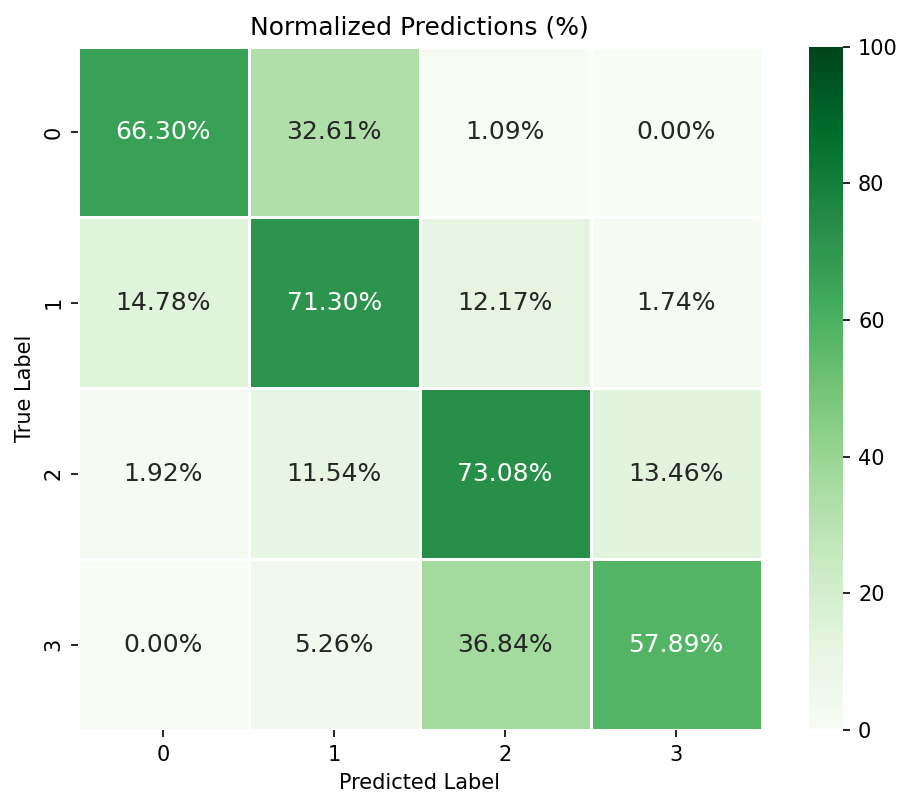
\includegraphics[width=\linewidth]{figures/fig7_.png}
    \caption{Row-normalized confusion matrix (\%) obtained on the held-out test images for the multi-region fusion model (ensemble + TTA).}
    \label{figmr}
\end{figure}

The multi-region fusion model reached 69.06\% accuracy, closing approximately 43\% of the gap between the region-crop result (64.18\%) and the whole-face upper bound (76.26\%), while its Quadratic Weighted Kappa (0.770) already slightly exceeds that of the region-crop model (0.718). This indicates that exploiting multiple regions of the same face, while preserving the anatomical embedding mechanism, recovers a substantial share of the benefit provided by full facial context in the whole-face baseline. This comes, however, at the cost of the region-localized output that is central to the proposed mobile application design (Fig.~\ref{figmobile}): the fusion model produces a single holistic estimate per image rather than an independent severity score per anatomical region. The two designs therefore address different use cases, and the choice between them should be guided by whether region-level granularity is required by the target application. Fig.~\ref{figmr} presents the corresponding row-normalized confusion matrix.



\section{Discussion}
Experimental results demonstrate that incorporating anatomical information enables a lightweight convolutional architecture to produce more ordinally consistent severity predictions than a conventional, region-agnostic ResNet-18, while preserving region-localized output and computational efficiency. Unlike approaches based on multiple specialized networks or computationally intensive architectures, the proposed framework enriches the visual representation with anatomical context while retaining a single, shared ResNet-18 backbone. This design reduces architectural complexity, facilitates training and deployment, and makes the model particularly suitable for teledermatology applications on mobile devices.

The controlled ablation reported in Section \ref{sub-IV-b}, run under an identical protocol and explicitly verified to be free of data leakage at the image level (Section \ref{sub-III-a}), shows that the anatomical embedding does not measurably change raw accuracy or F1-score relative to a conventional ResNet-18, but consistently improves the Quadratic Weighted Kappa, both per seed and after ensembling. Beyond this improvement in ordinal consistency, the region-aware design provides anatomically localized predictions, an outcome that a conventional, single-output classifier cannot produce, and one directly aligned with the region-by-region reporting envisioned for the mobile application described below.

The cross-source analysis in Section IV-C shows that performance decreases substantially when the model is evaluated on an image source entirely absent from training, and that this degradation follows an interpretable pattern rather than uniform noise. This quantifies a realistic generalization gap that a single random split over a combined dataset would otherwise obscure, and reinforces that continued diversification of the training collection across acquisition conditions is the most direct path toward narrowing it.

Regional analysis (Section IV-D) further indicates that residual performance differences across facial regions track the amount of usable training data per region more closely than any architectural limitation, again pointing toward data collection, rather than model design, as the primary lever for further improvement. The whole-face baseline reported in Section \ref{sub-IV-f} corroborates this reading: under the identical protocol, removing the region-crop constraint alone recovers a substantial share of accuracy, indicating that the residual gap is attributable to the reduced visual context available to a single anatomical crop rather than to a deficiency of the proposed embedding mechanism. The multi-region fusion result reported in Section \ref{sub-IV-g} reinforces this interpretation from a different angle: simply exposing the model to more of the available context, while still routing it through the same anatomical embeddings, recovers close to half of the gap without any change to the underlying backbone or embedding mechanism.

To demonstrate the practical applicability of the proposed framework, a mobile application was developed using the Flutter framework. The application integrates the trained ResNet-18 model, offering an end-to-end workflow for the remote assessment of acne severity. As illustrated in Figure~\ref{figmobile}, the application guides the user through the entire assessment process. Screen (a) displays the initial interface, while (b) allows for the capture or selection of a facial image. The captured image is automatically pre-processed and prepared for inference, as shown in (c). Subsequently, the region-aware ResNet-18 model estimates the acne severity level per anatomical region, which is presented to the user in (d) alongside the classification result. Finally, screens (e) and (f) provide the complete assessment report and assessment history, enabling longitudinal monitoring of the patient's progress during treatment.

\begin{figure}[htbp]
    \centering
    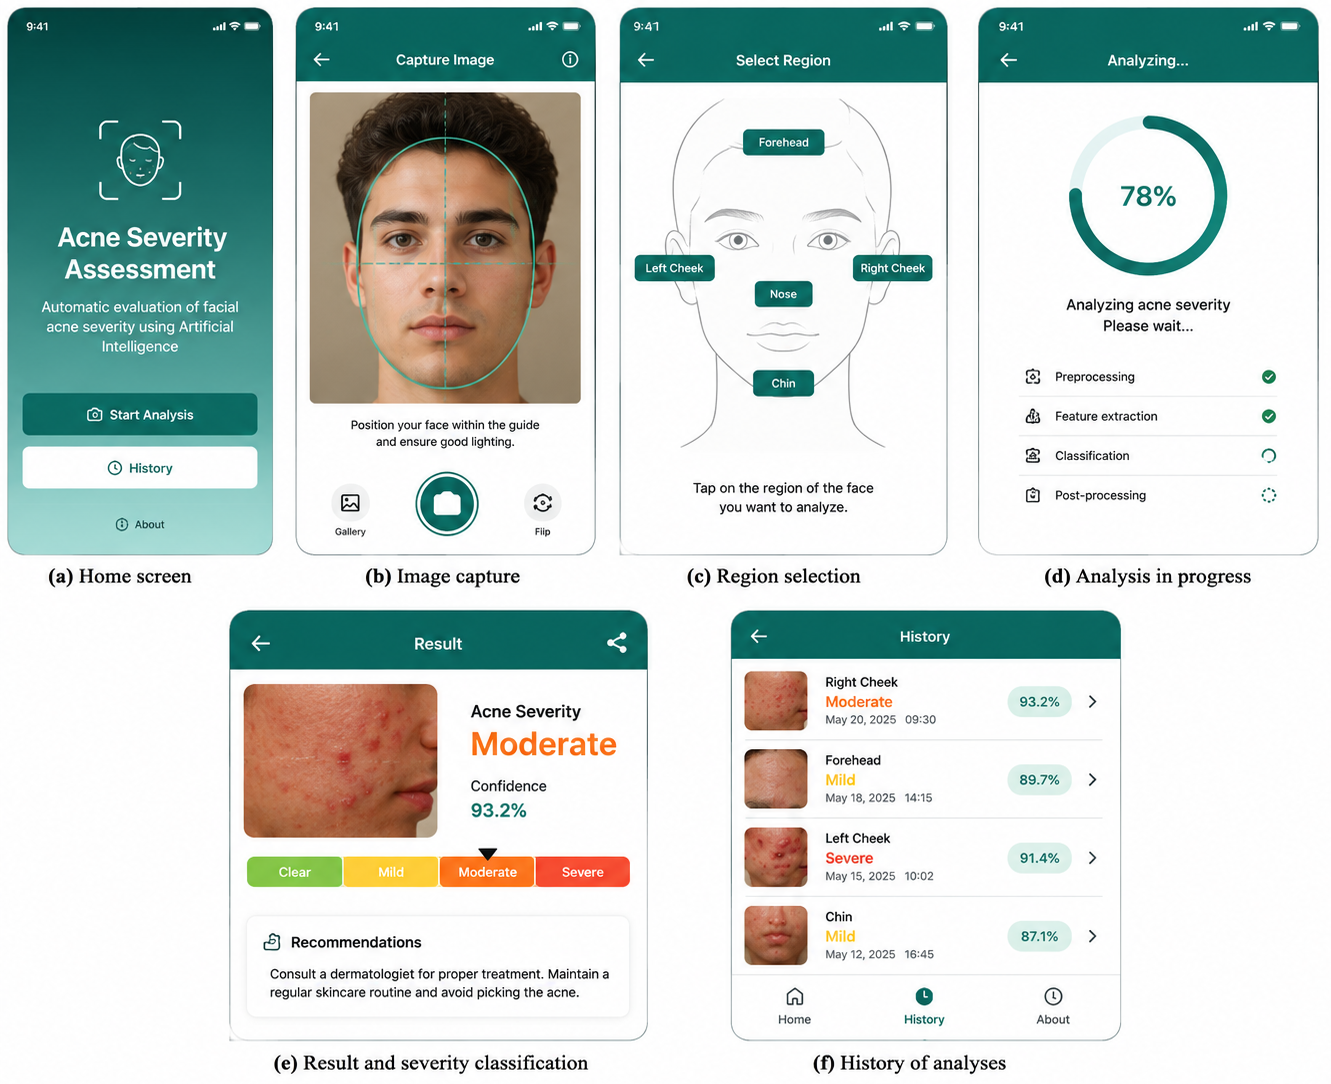
\includegraphics[width=\linewidth]{figures/fig6_.png}
    \caption{Flutter-based mobile prototype illustrating the complete teledermatology workflow: (a) home screen, (b) image acquisition, (c) preprocessing, (d) automatic acne severity prediction, (e) assessment report, and (f) evaluation history.}
    \label{figmobile}
\end{figure}

Although developed as a proof of concept, the mobile prototype demonstrates that the proposed architecture can be efficiently integrated into practical teledermatology systems, supporting remote patient monitoring while maintaining specialist oversight. Beyond facial acne severity classification, the proposed approach represents a general strategy for incorporating anatomical context into lightweight CNNs and may also benefit other biomedical image analysis tasks where anatomical location plays a significant role in clinical decision-making.


\section{Limitations}

Although the proposed framework achieved methodologically sound, ordinally more consistent predictions than its region-agnostic ablation baseline, several limitations must be considered. Most notably, the moderate absolute accuracy and the substantial cross-source generalization gap reported in Section IV-C indicate that the two image sources used in this study, while independently collected, still do not fully represent the diversity of patients, imaging devices, and acquisition conditions encountered in everyday clinical practice. Expanding the training collection toward a larger number of independent sources, and evaluating the proposed approach on additional held-out datasets, remains the most important step toward improving both absolute performance and generalizability.

Another aspect concerns the confidence estimates generated by the Softmax classifier, which were not explicitly calibrated in this study. Probability calibration and uncertainty estimation techniques could further enhance the framework's reliability, particularly given the ordinal nature of the severity scale and the observed sensitivity to distribution shift.

Finally, the mobile application developed using Flutter served as a proof of concept to demonstrate the practical feasibility of the proposed framework. Although the prototype replicates the entire inference workflow, it has not yet been validated in a clinical setting, and its underlying model reflects the accuracy levels reported in Section IV rather than the higher figures targeted in earlier stages of this work. Future studies should investigate its performance in real-world teledermatology contexts, considering different mobile devices, usability aspects, and longitudinal patient follow-up.

These limitations do not diminish the main contribution of this work. On the contrary, the controlled ablation and cross-source analyses were specifically designed to surface them, and they point directly to the next steps for transforming the proposed framework into a robust, clinically validated tool for AI-assisted teledermatology.


\section{Conclusion}
This study presented a region-aware ResNet-18 architecture for the automatic classification of facial acne severity, explicitly incorporating learnable anatomical region embeddings into a lightweight convolutional neural network. Unlike conventional lesion-based workflows or computationally intensive deep learning models, the proposed framework integrates anatomical context into a single shared backbone, offering an efficient solution for mobile teledermatology applications.

A controlled ablation showed that, under an identical, leakage-free protocol, the anatomical embedding does not change raw accuracy relative to a conventional ResNet-18 but consistently improves ordinal agreement (QWK), in addition to enabling the region-localized predictions that a conventional classifier cannot produce; a cross-source generalization analysis further quantified the model's behavior when evaluated on an independently collected image source entirely absent from training. An additional multi-region fusion variant showed that combining all available regions of the same image, while still exploiting the proposed anatomical embeddings, recovers close to half of the gap toward the whole-face upper bound, at the cost of the per-region output that the region-crop design provides. Together with the regional performance analysis, these experiments provide a more rigorous characterization of the proposed framework's behavior than a single in-distribution accuracy figure would allow. The development of a mobile prototype further demonstrated the practical feasibility of integrating the proposed approach into AI-assisted teledermatology workflows.

Future work will focus on expanding the training collection across additional independent sources and acquisition conditions to narrow the observed cross-source generalization gap, probability calibration, explainable AI techniques, and the prospective clinical evaluation of the proposed teledermatology system. Overall, the proposed framework represents a methodologically rigorous and efficient approach to AI-assisted facial acne severity assessment, whose main current limitation is the size and diversity of available annotated data rather than the architecture itself.

\section*{Acknowledgment}
The authors acknowledge the financial support provided by the Instituto Federal de Educação, Ciência e Tecnologia do Ceará (IFCE) through EDITAL Nº 9/2024 PRPI/REITORIA-IFCE, which made this research possible. The authors also thank the Laboratório de Processamento de Imagens e Simulação Computacional (LAPISCO) for providing the research infrastructure and scientific collaboration. In addition, the authors acknowledge the Conselho Nacional de Desenvolvimento Científico e Tecnológico (CNPq) for supporting one of the authors through a Master's scholarship.

\begin{thebibliography}{00}
\bibitem{b1} M. Vasam, A. Korivi, and K. M. Balli, “Acne vulgaris: A review of the pathophysiology, treatment, and recent nanotechnology-based advances,” Biomedicines, vol. 11, no. 12, Art. no. 3284, 2023.

\bibitem{b2} Y. Li, X. Hu, G. Dong, X. Wang, and T. Liu, “Acne treatment: research progress and new perspectives,” Frontiers in Medicine, vol. 11, Art. no. 1366957, 2024.

\bibitem{b3} G. D. Lenuța et al., “The epidemiology of acne in the current era: trends and clinical implications,” Cosmetics, vol. 12, no. 3, 2025.

\bibitem{b4} A. H. Heng and F. T. Chew, “Systematic review of the epidemiology of acne vulgaris,” Scientific Reports, vol. 10, Art. no. 5754, 2020.

\bibitem{b5} A. M. Layton, “The burden of acne vulgaris on health-related quality of life,” Dermatology and Therapy, vol. 15, 2025.

\bibitem{b6} D. V. Samuels, R. Rosenthal, R. Lin, S. Chaudhari, and M. N. Natsuaki, “Acne vulgaris and risk of depression and anxiety: A meta-analytic review,” Journal of the American Academy of Dermatology, vol. 83, no. 2, pp. 532–541, 2020.

\bibitem{b7} A. M. Layton, D. Thiboutot, and J. Tan, “Reviewing the global burden of acne: how could we improve care to reduce the burden?” British Journal of Dermatology, vol. 184, no. 2, pp. 219–225, 2021.

\bibitem{b8} A. S. Morshed et al., “Understanding the impact of acne vulgaris and associated psychological distress on self-esteem and quality of life,” Scientific Reports, vol. 13, Art. no. 15841, 2023.

\bibitem{b9} T. Tasneem et al., “Effects of acne severity and acne-related quality of life on depressive symptoms among adolescents and young adults,” Frontiers in Psychology, vol. 14, Art. no. 1213540, 2023.

\bibitem{b10} D. Z. Eichenfield, J. Sprague, and L. F. Eichenfield, “Management of acne vulgaris: a review,” JAMA, vol. 326, no. 20, pp. 2055–2067, 2021.

\bibitem{b11} S. Wongvibulsin et al., “Current state of dermatology mobile applications with artificial intelligence features,” JAMA Dermatology, vol. 160, no. 6, pp. 617–626, 2024.

\bibitem{b12} R. V. Reynolds et al., “Guidelines of care for the management of acne vulgaris,” Journal of the American Academy of Dermatology, vol. 90, no. 5, pp. 1006–1032, 2024.

\bibitem{b13} S. P. Choy, B. J. Kim, A. Paolino, W. R. Tan, S. M. L. Lim, J. Seo, S. P. Tan, and L. Francis, “Systematic review of deep learning image analyses for the diagnosis and monitoring of skin disease,” npj Digital Medicine, vol. 6, no. 1, Art. no. 180, 2023.

\bibitem{b14} Q. T. Huynh, P. H. Nguyen, H. X. Le, L. T. Ngo, N.-T. Trinh, M. T.-T. Tran, N. H. T. Nguyen, N. T. Vu, A. T. Nguyen, K. Suda, and H. T. Ngo, “Automatic acne object detection and acne severity grading using smartphone images and artificial intelligence,” Diagnostics, vol. 12, no. 8, Art. no. 1879, 2022.

\bibitem{b15} Y. Lin, J. Jiang, Z. Ma, D. Chen, Y. Guan, H. You, X. Cheng, B. Liu, and G. Luo, “KIEGLFN: A unified acne grading framework on face images,” Computer Methods and Programs in Biomedicine, vol. 221, Art. no. 106911, 2022.

\bibitem{b16} S. Liu, Y. Fan, M. Duan, Y. Wang, G. Su, Y. Ren, L. Huang, and F. Zhou, “AcneGrader: An ensemble pruning of the deep learning base models to grade acne,” Skin Research and Technology, vol. 28, no. 5, pp. 677–688, 2022.

\bibitem{b17} H. Wen, W. Yu, Y. Wu, J. Zhao, X. Liu, Z. Kuang, and R. Fan, “Acne detection and severity evaluation with interpretable convolutional neural network models,” Technology and Health Care, vol. 30, no. 1, pp. 143–153, 2022.

\bibitem{b18} Y. Lin, J. Jiang, D. Chen, Z. Ma, Y. Guan, X. Liu, H. You, and J. Yang, “DED: Diagnostic evidence distillation for acne severity grading on face images,” Expert Systems with Applications, vol. 228, Art. no. 120312, 2023.

\bibitem{b19} P. K. Nguyen, T. D. Le, B. A. Nguyen, and P. A. Nguyen, “ACNE8M: An acnes detection and differential diagnosis system using AI technologies,” VNUHCM Journal of Science and Technology Development, vol. 27, no. 3, pp. 3550–3561, 2024.

\bibitem{b20} L. Gazeau et al., “AcneAI: A new acne severity assessment method using digital images and deep learning,” in Proc. Int. Conf. Medical Image Computing and Computer-Assisted Intervention (MICCAI), 2024, pp. 68–78.

\bibitem{b21} N. Gao et al., “Evaluation of an acne lesion detection and severity grading model for Chinese population in online and offline healthcare scenarios,” Scientific Reports, vol. 15, Art. no. 1119, 2025.

\bibitem{b22} T. A. S. Viana, I. H. Gonçalves, I. S. Paula, F. H. S. Silva, and P. P. Rebouças Filho, “ClearFace: Facial acne detection and classification system using YOLOv11 and EfficientNet-B0,” in Proc. Conf. Graphics, Patterns and Images (SIBGRAPI) Extended Papers, 2025.

\bibitem{b23} K. He, X. Zhang, S. Ren, and J. Sun, “Deep residual learning for image recognition,” in Proc. IEEE Conf. Computer Vision and Pattern Recognition (CVPR), 2016, pp. 770–778.

\bibitem{b24} A. Paszke et al., “PyTorch: An imperative style, high-performance deep learning library,” in Advances in Neural Information Processing Systems (NeurIPS), vol. 32, 2019.

\bibitem{b25} C. Lugaresi et al., “MediaPipe: A framework for building perception pipelines,” arXiv preprint arXiv:1906.08172, 2019.

\bibitem{b26} A. G. C. Pacheco et al., “SCIN: A publicly available dataset for skin condition image analysis,” Google Research / Stanford Medicine, 2024.

\bibitem{b27} M. Hettich, “ACNE04 dataset,” Aug. 2019. [Online]. Available: https://www.kaggle.com/datasets/manuelhettich/acne04

\bibitem{b28} Flutter Documentation, “Flutter documentation,” 2026. [Online]. Available: https://docs.flutter.dev

\bibitem{b29} P. Izmailov, D. Podoprikhin, T. Garipov, D. Vetrov, and A. G. Wilson, “Averaging weights leads to wider optima and better generalization,” in Proc. Conf. Uncertainty in Artificial Intelligence (UAI), 2018.

\end{thebibliography}


\end{document}
